\section{Data formatting}\label{sec:formatting}
In this section, different ways to format and serialize RDF data are discussed. RDF data can be formatted into multiple formats, such as RDF/XML\cite{manola2004rdf}, RDFa\cite{herman2015rdfa}, Turtle\cite{beckett2014rdfturtle}, N-Triples\cite{beckett2014rdfntriples} and JSON-LD\cite{sporny2012json}. Each of these formats have their advantages and drawbacks, a detailed comparison is provided further in this section. Additionally, it is possible to receive data from various sources, such as databases. This section elaborates how this data can be transformed into RDF data so that it can be used for Linked Data querying.

\subsection{Resource Description Format (RDF)}\label{ssec:formatting-RDF}
Before considering the different formats to serialize RDF data, the RDF framework is described. The purpose of RDF is to create a general method to describe resources and relations between data objects, without making any assumptions regarding the domain. The concept of RDF originates from the problem that the World Wide Web was made to be interpreted by humans instead of machines. RDF proves to be an effective way of integrating information of different sources by decoupling the information from its original scheme. In other words, RDF aims to make the Web interpretable by machines\cite{lassila1998resource}.\\

\noindent One of the new features introduced in RDF 1.1\footnote{\url{https://www.w3.org/TR/rdf11-concepts/}} is the concept of named graphs. Since RDF 1.1, an RDF dataset may have multiple named graphs and at most one unnamed default graph. This enables grouping the data and as such giving extra context about how certain elements of the data are related \cite{schreiber2014rdf}. Subsequently, named graphs make it possible to both assign a URI to a collection of triples, and to create statements on the whole set.

\subsection{Data model}
\begin{figure}[htbp!]
    \centering
    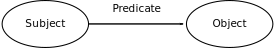
\includegraphics[width=\textwidth]{images/spo.pdf}
    \caption{Visualization of an RDF triple as a directed graph. This shows how a triple connects two labeled graph nodes via a directed labeled edge.}
    \label{fig:spo}
\end{figure}

\noindent RDF is structured as a collection of triples. These triples can be visualized as a node-arc-node link, which consists of a subject, a predicate, and an object (\Cref{fig:spo}). Thus this collection of triples can be interpreted as a graph, with the arc pointing towards the object \cite{klyne2009resource}.\\

\noindent An RDF triple represents a simple sentence. A commonly used example is the triple (\texttt{Alice - Knows - Bob}), which means that the subject ``Alice'', knows the object of the triple ``Bob''.

\subsection{Serialization format}
When reasoning about RDF, it is important to note that RDF itself is not a data format, but a data model. This model describes that the data should be represented as a triple, in the form of \texttt{subject - predicate - object}. Hence, to publish an RDF graph, it must be serialized using an RDF syntax\cite{heath2011linked}. Some of the standardized syntaxes are described below, each with the corresponding notation of the \texttt{Alice - Knows - Bob} example.

\subsubsection{RDF/XML}
The \emph{RDF/XML} syntax is the original RDF serialization format to publish Linked Data on the web. This syntax presents the RDF data model using XML (\Cref{lst:rdfxml-example}). However, the popularity of this syntax is decreasing, because it is difficult for humans to interpret and write \cite{manola2004rdf}.

\lstinputlisting[caption={RDF/XML representation of the \texttt{Alice - Knows - Bob} example},label=lst:rdfxml-example]{snippets/rdfxml_example.xml}

% Prevent widow.
\newpage

\subsubsection{Turtle and TriG}
\emph{Turtle} is a serialization format for RDF data that exposes the data in plain text. This format provides prefixes for namespaces and other abbreviations. These prefixes are described at the top of the document. Additionally with Turtle, every triple has to end with either one of three defined suffixes. The first suffix is a comma (\texttt{,}). This suffix indicates that the next triple has the same \emph{subject} and \emph{predicate} as the current triple, requiring nothing but the object on the next line. Alternatively, when a triple ends in a semicolon (\texttt{;}), the next triple has the same subject (but a different predicate) as the current one. Finally, a triple can have a dot (\texttt{.}) as its suffix. This suffix signals that the following triple does not have anything in common with the current triple. The abbreviations of Turtle are non-mandatory. As far as legibility is concerned, Turtle is considered one of the most readable and writable formats \cite{beckett2014rdfturtle}. This is illustrated in \Cref{lst:turtle-example}.\\

\noindent TriG is an extension of Turtle. Just like Turtle, TriG defines a textual syntax for RDF that allows an RDF dataset to be written in a compact and natural text form. TriG extends the functionalities of Turtle by bringing the possibility to group triples into multiple graphs. Furthermore, these named graphs (as described in \Cref{ssec:formatting-RDF}) can be preceded by their names. This is so important because named graphs are a key concept of the Semantic Web \cite{trig}. 

\lstinputlisting[caption={Turtle representation of the \texttt{Alice - Knows - Bob} example, from W3.org (\url{https://www.w3.org/TR/turtle/}).},label=lst:turtle-example]{snippets/turtle_example.ttl}

\subsubsection{N-Triples}
The N-Triples format (visualized in \Cref{lst:ntriples-example}) is a subset of Turtle that lacks support for prefixes and abbreviations. Consequently, this format is susceptible to both redundancies and larger file sizes when compared to Turtle. However, this redundancy also has an advantage: it allows line-by-line processing of N-Triples files. This allows for random access, straightforward compression, and usage in streaming contexts. Currently, the format is mostly used for files that are too big to fit into memory \cite{beckett2014rdfntriples}.

\lstinputlisting[caption={N-Triples representation of the \texttt{Alice - Knows - Bob} example.},label=lst:ntriples-example]{snippets/ntriples_example.txt}

\subsubsection{JSON-Linked Data (JSON-LD)}\label{sssec:formatting-jsonld}
JSON-LD is a lightweight Linked Data format, based on the widely used JavaScript Object Notation (JSON) format for formatting data. Because of this and because of its popularity, legibility, and writability, JSON-LD is the ideal format to pass Linked Data in a programming environment. Because JSON-LD uses the same syntax as JSON, it can easily be used to parse and manipulate RDF data \cite{sporny2012json}. An example of this syntax is provided in \Cref{lst:jsonld-example}.

% Prevent widow.
\clearpage

\lstinputlisting[caption={JSON-LD representation of the \texttt{Alice - Knows - Bob} example.},label=lst:jsonld-example]{snippets/jsonld_example.json}

\subsubsection{RDF in webpages}
Multiple formats can be used to embed RDF triples into existing webpages on the internet. The first format is RDFa, which integrates RDF triples into Hypertext Markup Language (HTML) documents by binding the RDF triples with the HTML Document Object Model (DOM). This means that the existing content of pages is shown, thanks to RDFa, inside the HTML code. Because of this, the structured data is exposed to the web \cite{herman2015rdfa}, as shown in \Cref{lst:rdfa-example}.

\lstinputlisting[caption={RDFa representation of the \texttt{Alice - Knows - Bob} example.},label=lst:rdfa-example]{snippets/rdfa_example.html}

\noindent Another option is to use Microdata. This format augments HTML webpages with specific machine-readable labels. It allows nested groups (items) of name-value pairs to be added to documents in addition to the existing content. To create an item, the \texttt{itemscope} attribute is used. An extra property can be added to an item with the \texttt{itemprop} attribute \cite{microdata}. This practice is demonstrated in \Cref{lst:microdata-example}.

\lstinputlisting[caption={Microdata representation of the \texttt{Alice - Knows - Bob} example.},label=lst:microdata-example]{snippets/microdata_example.html}

\noindent JSON-LD (\cref{sssec:formatting-jsonld}) snippets can be used to structure data into HTML as well. This method uses a JavaScript notation, embedded in a \texttt{script} tag. In other words, within the \texttt{script} tag, additional data can be represented in a structured format, using JSON-LD.

\subsubsection{Comma-Separated Values (CSV) on the web}
CSV is a popular format for publishing data. It is understandable by both humans and machines and it is typically presented in a table because of its structured format. Additionally, CSV data can easily be transformed into RDF data. However, one of the disadvantages of CSV is the absence of a mechanism to indicate the datatype of a specific column, which makes the data hard to validate. CSV on the Web solves this problem by augmenting the dataset with metadata that allows the publisher to provide additional information about the data \cite{tennison2016csv}. \Cref{lst:csvw-example} illustrates how the format of a country code field can be specified.

\lstinputlisting[caption={CSV on the Web example of a country code field specification, from W3.org (\url{https://www.w3.org/TR/tabular-data-primer/}).},label=lst:csvw-example]{snippets/csvw_example.json}

\subsubsection{Protocol Buffers}
Protocol Buffers are a technique developed by Google, designed for serializing structured data. Protocol Buffers aim to offer an interface description language for data, which is both simple and offers high performance. The data structures (referred to as messages) and services are described in ``proto definition files'', which are programming language-agnostic. Subsequently, Google provides code generators that allow generating source code in multiple different programming languages from these definition files. To achieve high performance, the messages are serialized into a binary format for transmission. This makes them both compact and forward- and backward-compatible. Backward compatibility means that a change in the technology will not break older versions. Forward compatibility on the other hand, means that a file from a more recent version can still be processed by older versions. A disadvantage of Protocol Buffers might be that it was developed for internal use, thus it was not optimized for unpredictable data (such as Linked Data) \cite{protobuf}.\\

\noindent In addition to Protocol Buffers, Google has also developed Flat Buffers. These offer access to the serialized data without requiring parsing or unpacking. Furthermore, Flat Buffers focus on memory efficiency, speed, flexibility, a tiny code footprint, strong types and ease-of-use. Flat Buffers work with cross-platform code without dependencies. However, this technology does not seem very useful for Linked Data, because it conflicts with the key principles of Linked Data by enforcing a scheme. Therefore, this is not further discussed in this paper \cite{flatbuf}.

\subsubsection{Header Dictionary Triples (HDT)}\label{sssec:formatting-hdt}
HDT is a binary format to represent RDF data in a compact way. An HDT file combines three parts. The first part is the header, which provides metadata about the dataset in a plain RDF format. The second part is the dictionary, which brings a mapping between strings and unique identifiers. The last part contains the triples and encodes the RDF graph using unique identifiers \cite{hdt}.

\subsection{RDF*}
RDF* (pronounced as ``RDF star'') is an extension to the Resource Description Framework, which enables RDF graphs to represent interactions and attributes by embedding triples. By nesting triples, an entire triple can become the subject of a second triple. This eliminates the need for intermediary entities, making the model easier to understand. Even though RDF* offers many benefits, it is still under consideration by the W3C and is not yet officially accepted as a standard.

\subsection{Decoupling data}\label{formatting-decoupling}
Since RDF is used to decouple data from its scheme, it should be possible to receive an arbitrary dataset (structured as e.g. CSV, XML, JSON or in a database), and transform this into an RDF format. To facilitate this, the RDF Mapping Language (RML) is used to materialize data into RDF triples.\\

\noindent RML is defined to express customized mapping rules from heterogeneous data structures and serializations to the RDF data model. Furthermore, RML is a superset of the W3C-standardized mapping language (R2RML). RML provides a generic way of defining the mappings that is easily transferable to cover references to other data structures. Thus, RML is a generic approach, but offers case-specific extensions. This makes it possible to transform any input (e.g., CSV, JSON, relational databases, etc.) into RDF data \cite{dimou2014rml}.
